\documentclass[amssymb,twocolumn,aps]{revtex4-2}
% allows special characters (including æøå)
\usepackage[utf8]{inputenc}
%\usepackage [norsk]{babel} %if you write norwegian
\usepackage[english]{babel}  %if you write english
\usepackage{array}
\usepackage{physics,amssymb}  % mathematical symbols (physics imports amsmath)
\usepackage{graphicx}         % include graphics such as plots
\usepackage[table]{xcolor}
\usepackage{xcolor}           % set colors
\usepackage{hyperref}         % automagic cross-referencing 
\usepackage{float}			  % force placement of tables and figures
\usepackage{textcomp}
\usepackage{tabularx}
\usepackage{amsmath, amssymb}
\usepackage{quantikz}
\usepackage{braket}
\usepackage{tikz}
\usetikzlibrary{decorations.pathreplacing}
\usepackage[table]{xcolor}
\usepackage{amssymb}
\usepackage{algorithm}
\usepackage{algpseudocode}
\usepackage{booktabs}
\usepackage{xcolor}
\usepackage{array}
\usepackage{float}
\usepackage{hyperref} 
\newtheorem{definition}{Definition}[section]
\usepackage{xcolor}
\usetikzlibrary{arrows.meta, positioning,  decorations.pathmorphing}
\usetikzlibrary{shapes.geometric, patterns, calc, positioning, shadows}

% Define color palette matching the schematic
\definecolor{izblue}{RGB}{0, 150, 230}
\definecolor{mzgreen}{RGB}{0, 153, 51}
\definecolor{szlightgreen}{RGB}{140, 200, 60}
\definecolor{regblue}{RGB}{70, 160, 245}
\definecolor{regred}{RGB}{255, 75, 60}
\definecolor{browntext}{RGB}{139, 35, 35}
\definecolor{cyanarrow}{RGB}{0, 200, 230}
\definecolor{panelbg}{RGB}{235, 238, 242}
\begin{document}
\title{Quantum Error Correction for the Neutral Atom Architecture}
\author{Jørgen Vestly \& Kristoffer Stalker}
\date{September 2026}
\begin{abstract}
      Neutral-atom arrays bound in optical tweezers present a compelling platform for fault-tolerant quantum error correction (QEC). Characterized by long coherence times in ground hyperfine states and strong, tunable van der Waals interactions during Rydberg excitations, neutral atoms enable scalable multi-qubit entangling gates. Furthermore, optical shuttling via acousto-optic deflectors allows non-local connectivity and dynamic lattice reconfigurations, enabling efficient surface code operations, lattice surgery, and erasure conversion. This overview outlines the hardware physics, open-system noise profiles, QEC code mappings, and real-time compilation strategies required for fault-tolerant neutral-atom quantum processors. FORELØPIG AI GENERERT ABSTRACT SÅ DONT MIND
\end{abstract}
\vspace{1.5em}
\maketitle
REMARKS: Skrev litt teori om QEC, la inn noe jeg har skrevet i 5429 og fylte på noe, men er ikke fullstendig ennå... jobber med det.
\section{Introduction}
Something motivational... like a Winston Chruchill quote or something - HER: \url{https://www.youtube.com/watch?v=GP-vIk2_TPk} Great one, m8!
\section{Background}
\subsection{Neutral Atoms as a Quantum Computer}
Describe the architecture: how does simple operations such as gates work on the platform, and how do they in turn make up a quantum computer? Explain Rydberg states as the unit of computation, and the different mechanisms ..\\\\
A \textit{neutral atom} is an atom with net zero electric charge (need ref.). More specifically, such atoms has an equal amount of protons and electrons. These atoms are especially favorable since they exhibit no coloumb interaction, and therefore making them robust against external electric and magnetic fields (neef ref.). Thus, their neutrality makes them easier to control and manipulate, a necessity for quantum computing.
\subsubsection{Rydberg states}
To create the computational unit in a quantum computer, a qubit, we use 
\begin{figure}[htbp]
  \centering
  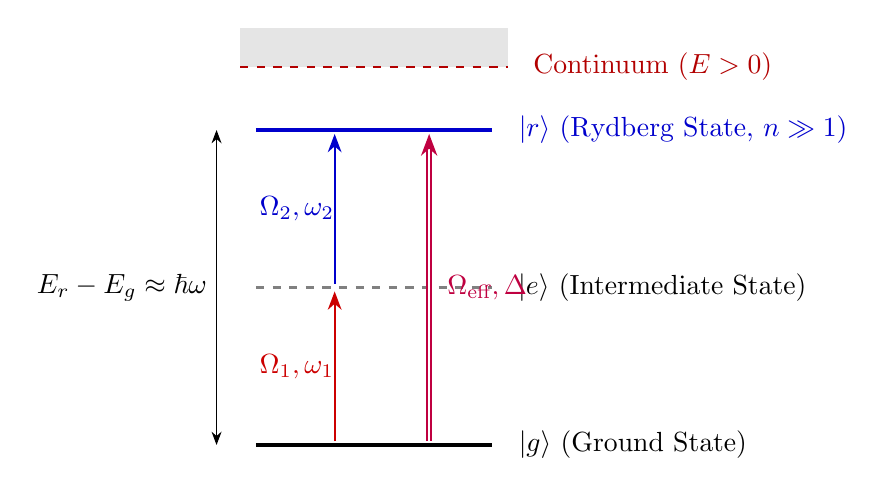
\begin{tikzpicture}[scale=1, >=Stealth]

    % Energy levels
    % Ground state |g>
    \draw[very thick, black] (0, 0) -- (3, 0) node[right=2mm] {$|g\rangle$ (Ground State)};
    
    % Intermediate state |e> (optional/virtual or real)
    \draw[thick, dashed, gray] (0, 2) -- (3, 2) node[right=2mm, black] {$|e\rangle$ (Intermediate State)};
    
    % Rydberg state |r>
    \draw[very thick, blue!80!black] (0, 4) -- (3, 4) node[right=2mm] {$|r\rangle$ (Rydberg State, $n \gg 1$)};

    % Ionization threshold
    \fill[gray!20] (-0.2, 4.8) rectangle (3.2, 5.3);
    \draw[dashed, red!70!black] (-0.2, 4.8) -- (3.2, 4.8) node[right=2mm] {Continuum ($E > 0$)};

    % Laser Transitions
    % First photon / drive (e.g. 780 nm)
    \draw[->, wave, thick, red!80!black] (1, 0.05) -- (1, 1.95) 
      node[midway, left=1mm] {$\Omega_1, \omega_1$};
      
    % Second photon / drive (e.g. 480 nm)
    \draw[->, wave, thick, blue!80!black] (1, 2.05) -- (1, 3.95) 
      node[midway, left=1mm] {$\Omega_2, \omega_2$};

    % Effective Two-Photon Rabi Frequency Arrow
    \draw[->, double, thick, purple] (2.2, 0.05) -- (2.2, 3.95) 
      node[midway, right=1mm] {$\Omega_{\text{eff}}, \Delta$};

    % Energy spacing annotations

\draw[<->] (-0.5, 0) -- (-0.5, 4)
    node[midway, left] {$E_r - E_g \approx \hbar\omega$};


  \end{tikzpicture}
  \caption{Energy level diagram of an alkali atom driven from ground state $|g\rangle$ to a high principal quantum number Rydberg state $|r\rangle$ via a two-photon laser excitation with effective Rabi frequency $\Omega_{\text{eff}}$ and detuning $\Delta$.}
  \label{fig:rydberg_energy_levels}
\end{figure}
\begin{figure}[htbp]
\centering
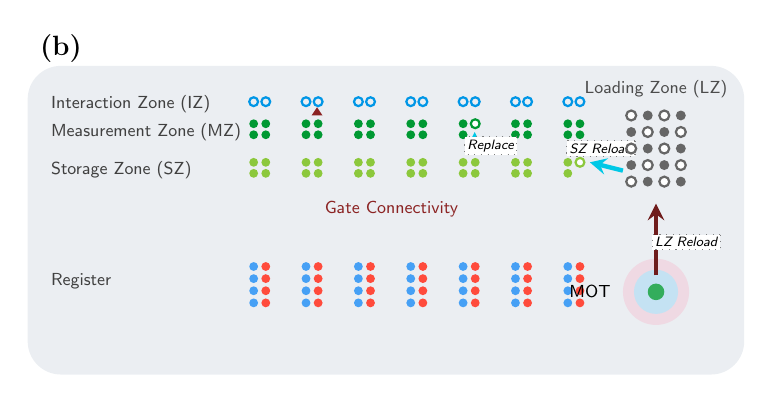
\begin{tikzpicture}[x=1cm, y=1cm, >=stealth, scale=0.7, transform shape]

    % Define local colors if not declared in main preamble
    \providecolor{izblue}{RGB}{0, 150, 230}
    \providecolor{mzgreen}{RGB}{0, 153, 51}
    \providecolor{szlightgreen}{RGB}{140, 200, 60}
    \providecolor{regblue}{RGB}{70, 160, 245}
    \providecolor{regred}{RGB}{255, 75, 60}
    \providecolor{browntext}{RGB}{139, 35, 35}
    \providecolor{cyanarrow}{RGB}{0, 200, 230}
    \providecolor{panelbg}{RGB}{235, 238, 242}

    % --- Outer Gray Panel ---
    \fill[panelbg, rounded corners=12pt] (-0.8, -0.6) rectangle (12.2, 5.0);
    
    % Panel Label (b)
    \node[anchor=north west, font=\bfseries\Large] at (-0.7, 5.7) {(b)};

    % --- ZONE LABELS (LEFT) ---
    \node[anchor=west, font=\sffamily\small, text=black!75] at (-0.5, 4.3) {Interaction Zone (IZ)};
    \node[anchor=west, font=\sffamily\small, text=black!75] at (-0.5, 3.8) {Measurement Zone (MZ)};
    \node[anchor=west, font=\sffamily\small, text=black!75] at (-0.5, 3.1) {Storage Zone (SZ)};
    \node[anchor=west, font=\sffamily\small, text=black!75] at (-0.5, 1.1) {Register};

    % --- REPEATING ATOM CLUSTERS (Columns 0 to 6) ---
    \foreach \col in {0,1,2,3,4,5,6} {
        \pgfmathsetmacro{\x}{3.3 + \col*0.95}

        % 1. Interaction Zone (IZ) - Open Blue Rings
        \draw[izblue, thick] (\x, 4.35) circle (0.08cm);
        \draw[izblue, thick] (\x+0.22, 4.35) circle (0.08cm);

        % 2. Measurement Zone (MZ) - 2x2 Dark Green Circles
        \fill[mzgreen] (\x, 3.95) circle (0.08cm);
        \fill[mzgreen] (\x+0.22, 3.95) circle (0.08cm);
        \fill[mzgreen] (\x, 3.75) circle (0.08cm);
        \ifnum\col=4
            \draw[mzgreen, thick, fill=white] (\x+0.22, 3.95) circle (0.08cm);
        \else
            \fill[mzgreen] (\x+0.22, 3.75) circle (0.08cm);
        \fi

        % 3. Storage Zone (SZ) - 2x2 Light Green Circles
        \fill[szlightgreen] (\x, 3.25) circle (0.08cm);
        \fill[szlightgreen] (\x+0.22, 3.25) circle (0.08cm);
        \fill[szlightgreen] (\x, 3.05) circle (0.08cm);
        \ifnum\col=6
            \draw[szlightgreen, thick, fill=white] (\x+0.22, 3.25) circle (0.08cm);
        \else
            \fill[szlightgreen] (\x+0.22, 3.05) circle (0.08cm);
        \fi

        % 4. Register - 4x2 Blue and Red Circles
        \foreach \row in {0,1,2,3} {
            \fill[regblue] (\x, 0.7 + \row*0.22) circle (0.08cm);
            \fill[regred]  (\x+0.22, 0.7 + \row*0.22) circle (0.08cm);
        }
    }

    % --- GATE CONNECTIVITY ANNOTATION ---
    \node[font=\sffamily\small, text=browntext] at (5.8, 2.4) {Gate Connectivity};
    \fill[browntext] (4.45, 4.25) -- (4.35, 4.10) -- (4.55, 4.10) -- cycle;

    % --- ANNOTATION: "Replace" ---
    \draw[cyanarrow, ->, ultra thick] (7.31, 3.4) -- (7.31, 3.8);
    \node[draw=gray, fill=white, inner sep=1.5pt, font=\sffamily\scriptsize\itshape, dotted] at (7.6, 3.55) {Replace};

    % --- ANNOTATION: "SZ Reload" ---
    \draw[cyanarrow, ->, ultra thick] (10.0, 3.1) -- (9.4, 3.25);
    \node[draw=gray, fill=white, inner sep=1.5pt, font=\sffamily\scriptsize\itshape, dotted] at (9.6, 3.5) {SZ Reload};

    % --- LOADING ZONE (LZ) ---
    \node[anchor=south, font=\sffamily\small, text=black!70] at (10.6, 4.3) {Loading Zone (LZ)};
    
    % 5x4 Array of Mixed Gray/White Circles (Fixed PGF logic)
    \foreach \r in {0,1,2,3,4} {
        \foreach \c in {0,1,2,3} {
            \pgfmathsetmacro{\lx}{10.15 + \c*0.3}
            \pgfmathsetmacro{\ly}{2.9 + \r*0.3}
            \pgfmathsetmacro{\isfilled}{mod(\r+\c, 2)}
            
            \ifdim \isfilled pt=0pt
                \draw[black!60, thick, fill=white] (\lx, \ly) circle (0.09cm);
            \else
                \fill[black!60] (\lx, \ly) circle (0.09cm);
            \fi
        }
    }

    % --- MOT & LZ RELOAD ---
    \fill[purple!20, opacity=0.6] (10.6, 0.9) circle (0.6cm);
    \fill[cyan!30, opacity=0.7] (10.6, 0.9) circle (0.4cm);
    \fill[mzgreen!80] (10.6, 0.9) circle (0.15cm);

    \node[anchor=east, font=\sffamily\small] at (9.9, 0.9) {MOT};

    % LZ Reload Arrow
    \draw[browntext!80!black, ->, ultra thick] (10.6, 1.2) -- (10.6, 2.5);
    \node[draw=gray, fill=white, inner sep=1.5pt, font=\sffamily\scriptsize\itshape, dotted] at (11.15, 1.8) {LZ Reload};

\end{tikzpicture}
\caption{Schematic representation of the neutral-atom architecture showcasing zonal transport, gate connectivity, and reload mechanisms.}

\label{fig:neutral_atom_architecture}
\end{figure}
\subsection{Quantum Error Correction}

So how would we implement a way to protect quantum information from noise, and assure that information is transmitted correctly through a quantum system? Quantum Error Correction is a set of techniques to protect information from noise in quantum systems, due to internal or external disturbances. As we have seen, quantum systems are inherently prone to noise and decoherence. Many of these errors are inevitable, and QEC does not prevent all errors from occurring, but instead detects them and applies corrections before they become logical errors. As we will see, the art of quantum error correction is to correct errors without measuring the qubits directly. This section will build up the intuition for doing QEC -- moving from error detection to error correction, exemplified through different \textit{error correcting codes} \cite{gottesman2024surviving,terhal2015quantum}.

\subsubsection*{Quantum channels and Pauli errors}

Before looking at QECCs (Quantum Error Correcting Codes), we must introduce the notion of a \textit{quantum channel}.
\begin{definition}[Quantum channel]
A quantum channel is a completely positive, trace-preserving (CPTP) map $\mathcal{N}$ acting on density operators $\rho$. It admits a Kraus representation
\begin{align*}
    \mathcal{N}(\rho)&=\sum_a A_a\rho A_a^\dagger, &
    \sum_a A_a^\dagger A_a&=I.
\end{align*}
The operators $A_a$ describe the possible error processes. The decomposition is not unique, but the linear span of the Kraus operators determines which errors a code must correct.
\end{definition}

We are particularly interested in \textit{Pauli errors}, described by the operators $\{I,X,Y,Z\}$, corresponding to no error, bit flip, bit-and-phase flip, and phase flip, respectively. A single-qubit Pauli channel takes the form
\begin{align*}
    \mathcal{N}_{P}(\rho)
    &=p_I\rho+p_XX\rho X
      +p_YY\rho Y+p_ZZ\rho Z,\\
    &\sum_{P\in\{I,X,Y,Z\}}p_P=1.
\end{align*}
Although a general quantum channel need not be a Pauli channel, Pauli operators form a basis for operators on qubits. Consequently, the correctability of a general error space can be analyzed through a spanning set of Pauli operators \cite{gottesman2024surviving,knill1997theory}. This is useful because stabilizer measurements reveal whether such errors have occurred without directly measuring the logical information.

\subsubsection*{The three-qubit repetition code}

We will, as many textbooks do, introduce the \textit{three-qubit repetition code} to illustrate the simple recipe for QEC \cite{nielsenchuang,gottesman2024surviving}. Circuit~\ref{fig:3_bit_code_encoder} encodes the information in an arbitrary qubit as
\begin{align*}
    \alpha\ket{0}+\beta\ket{1}
    &\longmapsto \alpha\ket{000}+\beta\ket{111},
\end{align*}
essentially \textit{repeating} the information three times. We further denote $\ket{000}$ and $\ket{111}$ by $\ket{0}_L$ and $\ket{1}_L$, respectively. The subscript $L$ refers to the logical state, corresponding to the initial one-qubit information.

\begin{figure}[t]
    \centering
    \[
    \begin{quantikz}
    \alpha\ket{0}+\beta\ket{1} & \ctrl{1} & \ctrl{2} & \qw \\
    \ket{0} & \targ{} & \qw & \qw \\
    \ket{0} & \qw & \targ{} & \qw
    \end{quantikz}
    \qquad\mapsto\qquad
    \alpha\ket{000}+\beta\ket{111}
    \]
    \caption{Encoding one logical qubit in the three-qubit repetition code.}
    \label{fig:3_bit_code_encoder}
\end{figure}

If one bit-flip error occurs in the encoded state, it can be corrected by applying the same Pauli operator again on the affected qubit. For instance, if the second qubit is flipped, we apply
\begin{align*}
    IXI\bigl(\alpha\ket{010}+\beta\ket{101}\bigr)
    &=\alpha\ket{000}+\beta\ket{111}.
\end{align*}
This error is called a \textit{bit-flip error}. A \textit{phase-flip error}, caused by $Z$, changes the relative phase of the state. The three-qubit repetition code in this basis protects against bit flips, while phase-flip errors require a similar construction in a rotated basis. The \textit{nine-qubit Shor code} combines these ideas and corrects arbitrary single-qubit errors \cite{shor1995scheme,nielsenchuang}. We will not dig into that particular code, but instead use the repetition code to establish the main principles.

As mentioned, the key idea of error correction is to detect errors without measuring the encoded qubit itself. The circuit in Fig.~\ref{fig:3_qubit_flip_code} uses two ancillary qubits to perform \textit{parity checks} on the data qubits. These checks determine whether two computational basis bits are equal or different. Mathematically,
\begin{align*}
    x\oplus y=0 &\quad\Longleftrightarrow\quad x=y,\\
    x\oplus y=1 &\quad\Longleftrightarrow\quad x\neq y,
    \qquad x,y\in\{0,1\}.
\end{align*}

\begin{figure}[t]
\centering
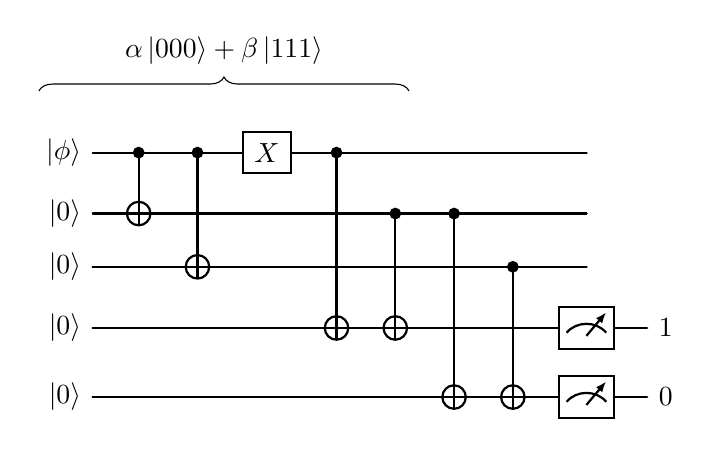
\begin{tikzpicture}
\node (circuit) {
\begin{quantikz}[column sep=0.42cm,row sep=0.35cm]
\lstick{$\ket{\phi}$} & \ctrl{1} & \ctrl{2} & \gate{X} & \ctrl{3} & \qw & \qw & \qw & \qw \\
\lstick{$\ket{0}$} & \targ{} & \qw & \qw & \qw & \ctrl{2} & \ctrl{3} & \qw & \qw \\
\lstick{$\ket{0}$} & \qw & \targ{} & \qw & \qw & \qw & \qw & \ctrl{2} & \qw \\
\lstick{$\ket{0}$} & \qw & \qw & \qw & \targ{} & \targ{} & \qw & \qw & \meter{} & \rstick{$1$} \\
\lstick{$\ket{0}$} & \qw & \qw & \qw & \qw & \qw & \targ{} & \targ{} & \meter{} & \rstick{$0$}
\end{quantikz}
};
\draw[decorate,decoration={brace,amplitude=5pt}]
  ([xshift=0.15cm,yshift=8pt]circuit.north west) --
  ([xshift=4.85cm,yshift=8pt]circuit.north west)
  node[midway,above=6pt] {$\alpha\ket{000}+\beta\ket{111}$};
\end{tikzpicture}
\caption{Syndrome extraction for the repetition code after an $X$ error on the first data qubit. The ancillas measure the two parities without revealing the logical amplitudes.}
\label{fig:3_qubit_flip_code}
\end{figure}

For example, an $X$ error on the first qubit produces
\begin{align*}
    \alpha\ket{000}+\beta\ket{111}
    &\longrightarrow
    \alpha\ket{100}+\beta\ket{011}.
\end{align*}
In plain language, the first qubit has flipped. The first parity check has odd parity, while the second has even parity, giving the bitstring $10$. This is an example of an \textit{error syndrome}: a collection of measurement outcomes indicating which parity checks have been violated. The corresponding recovery is determined by the syndrome, as summarized in Table~\ref{tab:three_qubit_syndromes}.

\begin{table}[t]
    \centering
    \caption{Syndromes and recovery operations for the three-qubit repetition code, assuming at most one $X$ error. The syndrome bits correspond to checks $ZZI$ and $IZZ$, respectively.}
    \label{tab:three_qubit_syndromes}
    \begin{tabular}{ccc}
        \toprule
        Error & Syndrome & Recovery \\
        \midrule
        $III$ & $00$ & $III$ \\
        $XII$ & $10$ & $XII$ \\
        $IXI$ & $11$ & $IXI$ \\
        $IIX$ & $01$ & $IIX$ \\
        \bottomrule
    \end{tabular}
\end{table}

For this simple example, the syndrome identifies the recovery uniquely. However, for larger codes the mapping between syndromes and errors need not be one-to-one. Different physical errors can produce the same syndrome, and successful correction is still possible if they act identically on the logical information. This property is known as \textit{degeneracy}. The correction conditions below make this distinction precise \cite{gottesman2024surviving,terhal2015quantum}.

\subsubsection*{Stabilizer codes}

One abstraction for defining QEC codes is to move away from a gate-by-gate description and instead define a code through its symmetries: parity-check operators that \textit{stabilize} all encoded states. This lets us describe the code algebraically, rather than through a particular circuit. Let $\mathcal{P}_n$ denote the $n$-qubit Pauli group, including its phase factors $\{\pm1,\pm i\}$. A \textit{stabilizer group} $\mathcal{S}\subseteq\mathcal{P}_n$ is an Abelian subgroup satisfying $-I\notin\mathcal{S}$ \cite{gottesman1997stabilizer,gottesman2024surviving,terhal2015quantum}.

If $\mathcal{S}=\langle S_1,\ldots,S_r\rangle$ has $r$ independent generators, its codespace is the common $+1$ eigenspace
\begin{align*}
    \mathcal{C}
    &=\{\ket{\psi}: S_i\ket{\psi}=\ket{\psi},
      \;i=1,\ldots,r\},\\
    [S_i,S_j]&=0\qquad\forall i,j.
\end{align*}
Its projector and dimension are
\begin{align*}
    \Pi_{\mathcal C}
    &=\prod_{i=1}^{r}\frac{I+S_i}{2},\\
    \dim\mathcal C&=2^{n-r}=2^k,
    \qquad k=n-r.
\end{align*}
Thus an $[[n,k]]$ stabilizer code encodes $k$ logical qubits into $n$ physical qubits.

For the three-qubit repetition code, the generators and stabilizer group are
\begin{align*}
    \mathcal S&=\langle ZZI,IZZ\rangle,\\
    &=\{III,ZZI,IZZ,ZIZ\}.
\end{align*}
All elements of the group are closed under multiplication; for example, $(ZZI)(IZZ)=ZIZ$ because $Z^2=I$. Hence two independent generators suffice to generate the entire group. The generators impose precisely the two parity conditions used above. If an error $E$ anticommutes with $S_i$, then for any $\ket{\psi}\in\mathcal C$,
\begin{align*}
    S_i E\ket{\psi}&=-E S_i\ket{\psi}
    =-E\ket{\psi}.
\end{align*}
Consequently, the measurement outcome of $S_i$ changes from $+1$ to $-1$. The associated syndrome bit is $1$; commuting errors produce a syndrome bit of $0$.

\subsubsection*{Error-correction conditions and code distance}

For an error set $\mathcal E=\{E_a\}$, a code with projector $\Pi_{\mathcal C}$ corrects every error in $\mathcal E$ if and only if the Knill--Laflamme conditions hold:
\begin{align*}
    \Pi_{\mathcal C}E_a^\dagger E_b\Pi_{\mathcal C}
    &=c_{ab}\Pi_{\mathcal C},
    \qquad E_a,E_b\in\mathcal E,
\end{align*}
where $c_{ab}$ is independent of the encoded state \cite{knill1997theory,gottesman2024surviving,nielsenchuang}.

For Pauli errors, this has a particularly simple stabilizer interpretation. For each pair $E_a,E_b\in\mathcal E$, the product $E_a^\dagger E_b$ must either be proportional to an element of $\mathcal S$, or anticommute with at least one stabilizer generator:
\begin{align*}
    E_a^\dagger E_b&\propto S\in\mathcal S,
    \quad\text{or}\\
    \exists S_i\in\mathcal S:\quad
    \{E_a^\dagger E_b,S_i\}&=0.
\end{align*}
The first case permits degenerate errors, whereas the second makes the corresponding error product detectable. In particular, a single Pauli operator $E$ is detectable if $E$ acts trivially on the code up to phase or anticommutes with a stabilizer generator.

The \textit{normalizer} of $\mathcal S$ within the Pauli group is
\begin{align*}
    \mathcal N(\mathcal S)
    &=\{P\in\mathcal P_n:[P,S]=0
       \;\forall S\in\mathcal S\}.
\end{align*}
Pauli operators in $\mathcal N(\mathcal S)$ preserve the codespace. Those not proportional to elements of $\mathcal S$ implement nontrivial logical operations. The \textit{code distance} is therefore
\begin{align*}
    d=\min_{\substack{P\in\mathcal N(\mathcal S)\\
                P\not\propto S\;\forall S\in\mathcal S}}
                \operatorname{wt}(P),
\end{align*}
where $\operatorname{wt}(P)$ is the number of qubits on which $P$ acts nontrivially. An $[[n,k,d]]$ code detects arbitrary Pauli errors of weight below $d$ and corrects arbitrary errors of weight at most $\lfloor(d-1)/2\rfloor$ \cite{terhal2015quantum,gottesman2024surviving}.

The repetition code illustrates the distinction between a restricted error model and general quantum errors: $XXX$ is a nontrivial logical bit flip of weight three, but $ZII$ is a nontrivial logical phase flip of weight one. Consequently, its full quantum parameters are $[[3,1,1]]$, despite its ability to correct one $X$ error.

\subsubsection*{Binary symplectic representation}

The stabilizer formalism admits a binary representation particularly suited to algebraic code construction. Ignoring global phases, every $n$-qubit Pauli operator can be written as
\begin{align*}
    P&\propto\bigotimes_{i=1}^{n}X_i^{x_i}Z_i^{z_i},\\
    \mathbf v(P)&=(\mathbf x\mid\mathbf z)
    \in\mathbb F_2^{2n},
\end{align*}
where $\mathbf x,\mathbf z\in\mathbb F_2^n$, with the local correspondence
\begin{align*}
    I&\leftrightarrow(0\mid0), &
    X&\leftrightarrow(1\mid0),\\
    Y&\leftrightarrow(1\mid1), &
    Z&\leftrightarrow(0\mid1).
\end{align*}
Here $\mathbb F_2=\{0,1\}$ is the binary field. Multiplication of Pauli strings, up to phase, becomes addition of their binary vectors modulo two.

The \textit{binary symplectic form} of $\mathbf v=(\mathbf x\mid\mathbf z)$ and $\mathbf w=(\mathbf x'\mid\mathbf z')$ is defined as
\begin{align*}
    \langle\mathbf v,\mathbf w\rangle_s
    &=\mathbf x\cdot\mathbf z'
      +\mathbf z\cdot\mathbf x'\pmod2\\
    &=\mathbf v J\mathbf w^T,\\
    J&=\begin{pmatrix}
        0&I_n\\ I_n&0
    \end{pmatrix}.
\end{align*}
It determines Pauli commutation through
\begin{align*}
    PQ=(-1)^{\langle\mathbf v(P),
                     \mathbf v(Q)\rangle_s}QP.
\end{align*}
In particular, $P$ and $Q$ commute precisely when their symplectic product vanishes \cite{gottesman2024surviving,calderbank1998quantum}.
\\\\
Let $H_{\mathcal S}\in\mathbb F_2^{r\times2n}$ be the \textit{stabilizer check matrix}, whose rows are the binary vectors of $S_1,\ldots,S_r$. Writing
\begin{align*}
    H_{\mathcal S}&=(H_X\mid H_Z),
\end{align*}
mutual commutation of the generators is equivalent to
\begin{align*}
    H_{\mathcal S}JH_{\mathcal S}^T=0\pmod2.
\end{align*}
For a Pauli error represented by $\mathbf e=(\mathbf x_e\mid\mathbf z_e)$, its syndrome is
\begin{align*}
    \mathbf s=H_{\mathcal S}J\mathbf e^T\pmod2.
\end{align*}
The $i$th component is one exactly when $E$ anticommutes with generator $S_i$.

For the repetition code, $H_X$ is zero and
\begin{align*}
    H_Z&=\begin{pmatrix}
       1&1&0\\
       0&1&1
    \end{pmatrix},\\
    \mathbf s&=H_Z\mathbf x_e^T\pmod2,
\end{align*}
recovering the two classical parity checks.
\\\\
A useful subclass is the Calderbank--Shor--Steane (CSS) family, in which the generators can be separated into purely $X$-type and purely $Z$-type checks. Denoting their binary support matrices by $H_X^{\mathrm{CSS}}$ and $H_Z^{\mathrm{CSS}}$, the commutation condition reduces to
\begin{align*}
    H_X^{\mathrm{CSS}}
    (H_Z^{\mathrm{CSS}})^T=0\pmod2.
\end{align*}
The $X$-type generators detect $Z$ errors, while $Z$-type generators detect $X$ errors \cite{calderbank1998quantum}. More generally, the symplectic representation provides a compact formulation of stabilizer commutation, error detection, and code construction in terms of binary constraints \cite{calderbank1998quantum}.

\subsection{SAT-based Code Design}
Something on SAT...\\
\begin{itemize}
    \item Define SAT discovery and extension
    \item Prerequisites for correct codes: mutual commutation etc
    \item Other theoretical considerations
\end{itemize}

\subsubsection{Hamiltonian- and Error-Informed Codes}
REASONING: Siden ikke alle Hamiltonians leder til symmetri, tenkte jeg det kunne være nyttig å definere forskjellen mellom H-koder direkte fra symmetri, og feil koder (epsilon-koder) uten krav til fysisk symmetri.
\begin{definition}[$H$-code]
Let $H=\sum_{\alpha}c_{\alpha}P_{\alpha}$ be a
Hamiltonian, and let
\begin{align*}
    \mathcal{G}_H
    =\{S\in\mathcal{P}_n:[S,H]=0\}
\end{align*}
denote its Pauli symmetry group.
An $H$-code is a stabilizer code obtained by
initializing SAT with a nontrivial commuting
subgroup $\mathcal{S}_0\subseteq\mathcal{G}_H$,
such that
\begin{align*}
    \mathcal{S}_0\subseteq\mathcal{S},
    \qquad
    \mathcal{S}=\langle S_1,\ldots,S_{n-k}\rangle,
\end{align*}
where $\mathcal{S}$ satisfies the prescribed
error-correction constraints for $\mathcal{E}$.
\end{definition}


\begin{definition}[$\mathcal{E}$-code]
Let $\mathcal{E}\subseteq\mathcal{P}_n$ denote a set
of Pauli error operators. An $\mathcal{E}$-code is
a stabilizer code obtained through SAT without
requiring any prior knowledge of Hamiltonian
symmetries, whose stabilizer group
$\mathcal{S}=\langle S_1,\ldots,S_{n-k}\rangle$
satisfies, for every $E\in\mathcal{E}$,
\begin{align*}
    E\in\mathcal{S}
    \quad\lor\quad
    \exists S_i\in\mathcal{S}:
    \{E,S_i\}=0.
\end{align*}
For correction of an error set $\mathcal{F}$,
this condition is imposed on all
$E=E_a^\dagger E_b$, where
$E_a,E_b\in\mathcal{F}$, with Pauli phases
understood modulo the stabilizer group.
\end{definition}


\subsection{Physics-informed Code Design for Neutral Atoms}
Btw subsection title might be altered here...Also, need an introduction to the subsection going from the abstract and general SAT solver to physics informed.
\subsubsection{The Model}
The dynamics of neutral atoms can be described by the Hamiltonian of the three-level Rydberg atom, given by
\begin{equation}
H = \frac{\hbar \Omega}{2} \sum_i \sigma_x^i
- \hbar \delta \sum_i n_i
+ \sum_{i<j} V_{ij} n_i n_j,
\qquad
\label{eq:qubit_rydberg_H}
\end{equation}
where $V_{ij} = \frac{C_6}{R_{ij}^6}.$ as described in \cite{Browaeys2020}. Our particular model for the Rydberg atom is described as a qutrit state, with basis states $\{\ket{g}, \ket{e}, \ket{r}\}$ as showed in Figure \ref{fig:rydberg_energy_levels}. In order to describe the full dynamics of the qutrit state, one must expland the general Hamiltonian in Equation \ref{eq:qubit_rydberg_H}, to consider the three possible states. This Hamiltonian is given by

\begin{equation}
\begin{aligned}
\frac{\mathcal{H}(t)}{\hbar}
={}&
\sum_i \frac{\Omega_i^{\mathrm{hf}}(t)}{2}
\left(
e^{i\phi_i^{\mathrm{hf}}(t)}
|0_i\rangle\langle 1_i|
+
e^{-i\phi_i^{\mathrm{hf}}(t)}
|1_i\rangle\langle 0_i|
\right)
\\
&-
\sum_i \Delta_i^{\mathrm{hf}}(t)
|1_i\rangle\langle 1_i|
\\
&+
\sum_i \frac{\Omega_i^{\mathrm{r}}(t)}{2}
\left(
e^{i\phi_i^{\mathrm{r}}(t)}
|1_i\rangle\langle r_i|
+
e^{-i\phi_i^{\mathrm{r}}(t)}
|r_i\rangle\langle 1_i|
\right)
\\
&-
\sum_i
\left[
\Delta_i^{\mathrm{hf}}(t)
+
\Delta_i^{\mathrm{r}}(t)
\right]
|r_i\rangle\langle r_i|
\\
&+
\sum_{i<j} V_{ij}
|r_i\rangle\langle r_i|
\otimes
|r_j\rangle\langle r_j|,
\end{aligned}
\label{eq:rydberg_three_level}
\end{equation}
where the superscripts \(\mathrm{hf}\) and \(\mathrm{r}\) denote the hyperfine and Rydberg transitions, respectively, where the former couples the computational states \(|0\rangle\) and \(|1\rangle\), while the latter couples \(|1\rangle\) to the excited Rydberg state \(|r\rangle\). The Rabi frequencies \(\Omega_i\) determine the strength of these couplings, \(\phi_i\) their phases, and \(\Delta_i\) the detuning from resonance. Finally, \(V_{ij}\) describes the interaction between atoms \(i\) and \(j\) when both occupy the Rydberg state, typically given by \(V_{ij}=C_6/R_{ij}^6\), where \(R_{ij}\) is the interatomic distance and \(C_6\) is the van der Waals interaction coefficient.\\\\
The Hamiltonian must be transformed into a sum of Pauli operators. Any hermitian Hamiltonian can be decomposed as
\begin{equation}
    H = \sum_\alpha c_\alpha P_\alpha, P \in \{\mathcal{I}, \mathcal{X}, \mathcal{Y}, \mathcal{Z}\}.
\end{equation}
We encode the basis states into two-qubit states, by the binary mapping
\begin{align*}
    \ket{0} \to \ket{00}\\
    \ket{1} \to \ket{01}\\
    \ket{r} \to \ket{11}.
\end{align*}
The Rydberg Hamiltonian in Eq. \ref{eq:rydberg_three_level}, can be rewritten as

\begin{align*}
    H &= H_{\mathrm{hf}} + H_{\Delta_{\mathrm{hf}}}
       + H_{\mathrm{r}} + H_{\Delta_{\mathrm{r}}} + H_V
\end{align*}

Then, we map the projectors to Pauli operators, by the convention given in Eq. 6 in \cite{Sawaya2020}, as

\begin{align*}
    \ket{0_i}\bra{1_i}
    &\mapsto \ket{00}_i\bra{01}
    = \ket{0}\bra{0}\otimes\ket{0}\bra{1}\\
    &= \frac{I+Z}{2}\otimes\frac{X+iY}{2}\\
    &= \frac{1}{4}(IX+iIY+ZX+iZY)_i,\\[8pt]
    \ket{1_i}\bra{0_i}
    &\mapsto \ket{01}_i\bra{00}
    = \ket{0}\bra{0}\otimes\ket{1}\bra{0}\\
    &= \frac{I+Z}{2}\otimes\frac{X-iY}{2}\\
    &= \frac{1}{4}(IX-iIY+ZX-iZY)_i.
\end{align*}
Thus, the first term can be rewritten as
\begin{align*}
    \frac{H_{\mathrm{hf}}}{\hbar}
    &= \sum_i \frac{\Omega_i^{\mathrm{hf}}}{8}
    \Big[
    e^{i\phi_i^{\mathrm{hf}}}
    (IX+iIY+ZX+iZY)_i\\
    &\qquad\qquad+
    e^{-i\phi_i^{\mathrm{hf}}}
    (IX-iIY+ZX-iZY)_i
    \Big]\\[6pt]
    &= \sum_i \frac{\Omega_i^{\mathrm{hf}}}{4}
    \Big[
    \cos\phi_i^{\mathrm{hf}}(IX+ZX)_i
    -\sin\phi_i^{\mathrm{hf}}(IY+ZY)_i
    \Big].
\end{align*}
Idk, kanskje gjøre dette litt mer clean? Regningen er riktig, men twocolumns er shit estesisk sett.
Following the same procedure for the other terms, we get the final decomposition
\begin{align*}
    \frac{H}{\hbar}
    ={}&
    \sum_i\frac{\Omega_i^{\mathrm{hf}}}{4}
    \Big[
        \cos\phi_i^{\mathrm{hf}}(IX+ZX)_i\\
    &\qquad
        -\sin\phi_i^{\mathrm{hf}}(IY+ZY)_i
    \Big]\\[4pt]
    &-\sum_i\frac{\Delta_i^{\mathrm{hf}}}{4}
      (II-IZ+ZI-ZZ)_i\\[4pt]
    &+\sum_i\frac{\Omega_i^{\mathrm{r}}}{4}
    \Big[
        \cos\phi_i^{\mathrm{r}}(XI-XZ)_i\\
    &\qquad
        -\sin\phi_i^{\mathrm{r}}(YI-YZ)_i
    \Big]\\[4pt]
    &-\sum_i
      \frac{\Delta_i^{\mathrm{hf}}+\Delta_i^{\mathrm{r}}}{4}
      (II-IZ-ZI+ZZ)_i\\[4pt]
    &+\sum_{i<j}\frac{V_{ij}}{16}
      (II-IZ-ZI+ZZ)_i\\
    &\qquad\qquad\otimes
      (II-IZ-ZI+ZZ)_j.
\end{align*}

\subsubsection{Hamiltonian Symmetries}
Given the Pauli decomposition of the Hamiltonian,
\begin{align*}
    H = \sum_{\alpha=1}^{m} c_\alpha P_\alpha,
    \qquad P_\alpha \in \mathcal{P}_n,
\end{align*}
we seek Pauli operators $S \in \mathcal{P}_n$
that commute with the Hamiltonian,
\begin{align*}
    [S,H] = 0.
\end{align*}

Since the distinct Pauli strings form a linearly
independent operator basis, this is equivalent to
\begin{align*}
    [S,P_\alpha] = 0,
    \qquad \forall \alpha \text{ with } c_\alpha \neq 0.
\end{align*}

Following the binary symplectic representation
\cite{Gottesman2026}, each $n$-qubit Pauli operator
is mapped to a binary vector,
\begin{align*}
    P_\alpha &\longleftrightarrow
    \mathbf{v}_\alpha =
    (\mathbf{x}_\alpha \mid \mathbf{z}_\alpha)
    \in \mathbb{F}_2^{2n},
\end{align*}
using
\begin{align*}
    I &\leftrightarrow (0,0),
    &X &\leftrightarrow (1,0),\\
    Y &\leftrightarrow (1,1),
    &Z &\leftrightarrow (0,1).
\end{align*}

Two Pauli operators commute if and only if their
symplectic product vanishes,
\begin{align*}
    \mathbf{v}_\alpha \odot \mathbf{s}
    &=
    \mathbf{x}_\alpha \cdot \mathbf{z}_S
    + \mathbf{z}_\alpha \cdot \mathbf{x}_S\\
    &= 0 \pmod 2,
\end{align*}
where $\mathbf{s}=(\mathbf{x}_S\mid\mathbf{z}_S)$
represents an unknown Pauli symmetry.

Collecting the binary representations of all
nonzero Pauli terms gives

\begin{align*}
    A_H &=
    \begin{pmatrix}
        \mathbf{x}_1 & \mathbf{z}_1 \\
        \mathbf{x}_2 & \mathbf{z}_2 \\
        \vdots & \vdots \\
        \mathbf{x}_m & \mathbf{z}_m
    \end{pmatrix}, \\[8pt]
    J &=
    \begin{pmatrix}
        0 & I_n \\
        I_n & 0
    \end{pmatrix}.
\end{align*}

The commutation conditions can therefore be
expressed as the linear system
\begin{align*}
    A_H J \mathbf{s}^{T}
    &= 0 \pmod 2.
\end{align*}

Defining $M_H=A_HJ$, the space of Pauli
symmetries is obtained from
\begin{align*}
    \mathbf{s} \in \ker_{\mathbb{F}_2}(M_H).
\end{align*}

The nullspace is computed through Gaussian
elimination over $\mathbb{F}_2$, avoiding
explicit enumeration of all $4^n$ Pauli
operators \cite{Nagpal2026}.

The resulting binary vectors are mapped back
to Pauli strings. A mutually commuting,
independent subset may then be selected as
candidate stabilizer generators, with the
appropriate symmetry eigenspaces specified.
\\\\
Fant ingen ikke-trivielle symmetrier for Hamiltonian'en... kun identitetsoperatorer. Målet er å prøve å skrive H om til et mangepartikkel uttrykk og gjøre en transformering...
\subsubsection{Transforming to the Lipkin model}
We have established that no H-codes can be retrieved from the former Hamiltonians. However, by transforming the orignal three-level Hamiltonian in Eq. \ref{eq:rydberg_three_level}, we can find non-trivial symmetries. We can prove that the three-level Rydberg atom has the same effective physics as the Lipkin-Meshkov-Glick model given by

\begin{equation}
\begin{aligned}
H_{\mathrm{LMG}}^{(3)}
={}&\frac{1}{N}
\left(
-\epsilon_0 T_{00}
+\epsilon_1 T_{11}
+\epsilon_r T_{rr}
\right)\\
&-\frac{\lambda}{N(N-1)}
\sum_{\substack{a,b\in\{0,1,r\}\\a\neq b}}
T_{ab}^{2},
\end{aligned}
\end{equation}
where $T_{ab}$ denotes the transition operators, defined as
\begin{equation*}
    T_{ab} = \sum_i^N \ket{a_i}\bra{b_i}.
\end{equation*}

\section{Methodology}
\section{Discussion}
\section{Conclusion and Future Outlook}
\appendix
\section{Pauli Decomposition of the Rydberg Hamiltonian}
\label{app:pauli_decomposition}

The three-level Rydberg Hamiltonian is separated into
five contributions:
\begin{align*}
    H &= H_{\mathrm{hf}}
       + H_{\Delta,\mathrm{hf}}
       + H_{\mathrm{r}}
       + H_{\Delta,\mathrm{r}}
       + H_V.
\end{align*}

The individual terms are
\begin{align*}
    \frac{H_{\mathrm{hf}}}{\hbar}
    &= \sum_i \frac{\Omega_i^{\mathrm{hf}}}{2}
    \left(
        e^{i\phi_i^{\mathrm{hf}}}\ket{0_i}\bra{1_i}
        + e^{-i\phi_i^{\mathrm{hf}}}\ket{1_i}\bra{0_i}
    \right), \\[6pt]
    \frac{H_{\Delta,\mathrm{hf}}}{\hbar}
    &= -\sum_i \Delta_i^{\mathrm{hf}}
       \ket{1_i}\bra{1_i}, \\[6pt]
    \frac{H_{\mathrm{r}}}{\hbar}
    &= \sum_i \frac{\Omega_i^{\mathrm{r}}}{2}
    \left(
        e^{i\phi_i^{\mathrm{r}}}\ket{1_i}\bra{r_i}
        + e^{-i\phi_i^{\mathrm{r}}}\ket{r_i}\bra{1_i}
    \right), \\[6pt]
    \frac{H_{\Delta,\mathrm{r}}}{\hbar}
    &= -\sum_i
       (\Delta_i^{\mathrm{hf}}+\Delta_i^{\mathrm{r}})
       \ket{r_i}\bra{r_i}, \\[6pt]
    \frac{H_V}{\hbar}
    &= \sum_{i<j} V_{ij}
       \ket{r_i}\bra{r_i}
       \otimes \ket{r_j}\bra{r_j}.
\end{align*}

\subsection*{Binary encoding}

Following the binary encoding of Sawaya et
al.~\cite{Sawaya2020}, the atomic states are mapped as
\begin{align*}
    \ket{0} &\longmapsto \ket{00},\\
    \ket{1} &\longmapsto \ket{01},\\
    \ket{r} &\longmapsto \ket{11}.
\end{align*}

The single-qubit operators are expressed as
\begin{align*}
    \ket{0}\bra{0} &= \frac{I+Z}{2},
    &\ket{1}\bra{1} &= \frac{I-Z}{2},\\[4pt]
    \ket{0}\bra{1} &= \frac{X+iY}{2},
    &\ket{1}\bra{0} &= \frac{X-iY}{2}.
\end{align*}

Here, $IX=I\otimes X$, $ZZ=Z\otimes Z$, etc.
Identity operators on the remaining atoms are implicit.

\subsection*{Hyperfine driving term}

The transition operators become
\begin{align*}
    \ket{0}\bra{1}
    &\longmapsto \ket{00}\bra{01}\\
    &= \ket{0}\bra{0}\otimes\ket{0}\bra{1}\\
    &= \frac{I+Z}{2}\otimes\frac{X+iY}{2}\\
    &= \frac14(IX+iIY+ZX+iZY),
    \\[8pt]
    \ket{1}\bra{0}
    &\longmapsto \ket{01}\bra{00}\\
    &= \ket{0}\bra{0}\otimes\ket{1}\bra{0}\\
    &= \frac{I+Z}{2}\otimes\frac{X-iY}{2}\\
    &= \frac14(IX-iIY+ZX-iZY).
\end{align*}

Substitution into the Hamiltonian gives
\begin{align*}
    \frac{H_{\mathrm{hf}}}{\hbar}
    &= \sum_i \frac{\Omega_i^{\mathrm{hf}}}{8}
    \Big[
        e^{i\phi_i^{\mathrm{hf}}}
        (IX+iIY+ZX+iZY)_i\\
    &\qquad\qquad
        +e^{-i\phi_i^{\mathrm{hf}}}
        (IX-iIY+ZX-iZY)_i
    \Big]\\[6pt]
    &= \sum_i \frac{\Omega_i^{\mathrm{hf}}}{4}
    \Big[
        \cos\phi_i^{\mathrm{hf}}(IX+ZX)_i\\
    &\qquad\qquad
        -\sin\phi_i^{\mathrm{hf}}(IY+ZY)_i
    \Big].
\end{align*}

\subsection*{Hyperfine detuning term}

The projector onto $\ket{1}$ becomes
\begin{align*}
    \ket{1}\bra{1}
    &\longmapsto \ket{01}\bra{01}\\
    &= \ket{0}\bra{0}\otimes\ket{1}\bra{1}\\
    &= \frac{I+Z}{2}\otimes\frac{I-Z}{2}\\
    &= \frac14(II-IZ+ZI-ZZ).
\end{align*}

Therefore,
\begin{align*}
    \frac{H_{\Delta,\mathrm{hf}}}{\hbar}
    &= -\sum_i\Delta_i^{\mathrm{hf}}
       \ket{1_i}\bra{1_i}\\
    &= -\sum_i\frac{\Delta_i^{\mathrm{hf}}}{4}
       (II-IZ+ZI-ZZ)_i.
\end{align*}

\subsection*{Rydberg driving term}

The transition operators become
\begin{align*}
    \ket{1}\bra{r}
    &\longmapsto \ket{01}\bra{11}\\
    &= \ket{0}\bra{1}\otimes\ket{1}\bra{1}\\
    &= \frac{X+iY}{2}\otimes\frac{I-Z}{2}\\
    &= \frac14(XI-XZ+iYI-iYZ),
    \\[8pt]
    \ket{r}\bra{1}
    &\longmapsto \ket{11}\bra{01}\\
    &= \ket{1}\bra{0}\otimes\ket{1}\bra{1}\\
    &= \frac{X-iY}{2}\otimes\frac{I-Z}{2}\\
    &= \frac14(XI-XZ-iYI+iYZ).
\end{align*}

Substituting into the Rydberg driving term,
\begin{align*}
    \frac{H_{\mathrm{r}}}{\hbar}
    &= \sum_i\frac{\Omega_i^{\mathrm{r}}}{8}
    \Big[
        e^{i\phi_i^{\mathrm{r}}}
        (XI-XZ+iYI-iYZ)_i\\
    &\qquad\qquad
        +e^{-i\phi_i^{\mathrm{r}}}
        (XI-XZ-iYI+iYZ)_i
    \Big]\\[6pt]
    &= \sum_i\frac{\Omega_i^{\mathrm{r}}}{4}
    \Big[
        \cos\phi_i^{\mathrm{r}}(XI-XZ)_i\\
    &\qquad\qquad
        -\sin\phi_i^{\mathrm{r}}(YI-YZ)_i
    \Big].
\end{align*}

\subsection*{Rydberg detuning term}

The projector onto $\ket{r}$ becomes
\begin{align*}
    \ket{r}\bra{r}
    &\longmapsto \ket{11}\bra{11}\\
    &= \ket{1}\bra{1}\otimes\ket{1}\bra{1}\\
    &= \frac{I-Z}{2}\otimes\frac{I-Z}{2}\\
    &= \frac14(II-IZ-ZI+ZZ).
\end{align*}

Hence,
\begin{align*}
    \frac{H_{\Delta,\mathrm{r}}}{\hbar}
    &= -\sum_i
       (\Delta_i^{\mathrm{hf}}+\Delta_i^{\mathrm{r}})
       \ket{r_i}\bra{r_i}\\
    &= -\sum_i
       \frac{\Delta_i^{\mathrm{hf}}+\Delta_i^{\mathrm{r}}}{4}
       (II-IZ-ZI+ZZ)_i.
\end{align*}

\subsection*{Rydberg interaction term}

The interaction between two atoms is
\begin{align*}
    \frac{H_V}{\hbar}
    &= \sum_{i<j}V_{ij}
       \ket{r_i}\bra{r_i}
       \otimes\ket{r_j}\bra{r_j}.
\end{align*}

Using the Rydberg projector,
\begin{align*}
    &\ket{r_i}\bra{r_i}
     \otimes\ket{r_j}\bra{r_j}\\
    &\quad\longmapsto
      \ket{11}_i\bra{11}
      \otimes\ket{11}_j\bra{11}\\
    &\quad=
      \frac14(II-IZ-ZI+ZZ)_i
      \otimes
      \frac14(II-IZ-ZI+ZZ)_j\\
    &\quad=
      \frac1{16}(II-IZ-ZI+ZZ)_i
      \otimes(II-IZ-ZI+ZZ)_j.
\end{align*}

Expanding the tensor product,
\begin{align*}
    &\ket{r_i}\bra{r_i}
     \otimes\ket{r_j}\bra{r_j}\\
    &\quad=
    \frac1{16}\Big(
       IIII-IIIZ-IIZI+IIZZ\\
    &\qquad\quad
       -IZII+IZIZ+IZZI-IZZZ\\
    &\qquad\quad
       -ZIII+ZIIZ+ZIZI-ZIZZ\\
    &\qquad\quad
       +ZZII-ZZIZ-ZZZI+ZZZZ
    \Big)_{ij}.
\end{align*}

Thus,
\begin{align*}
    \frac{H_V}{\hbar}
    &= \sum_{i<j}\frac{V_{ij}}{16}
       (II-IZ-ZI+ZZ)_i\\
    &\qquad\qquad\otimes
       (II-IZ-ZI+ZZ)_j.
\end{align*}

\subsection*{Complete Pauli decomposition}

Combining the five contributions yields
\begin{align*}
    \frac{H}{\hbar}
    ={}&
    \sum_i\frac{\Omega_i^{\mathrm{hf}}}{4}
    \Big[
        \cos\phi_i^{\mathrm{hf}}(IX+ZX)_i\\
    &\qquad
        -\sin\phi_i^{\mathrm{hf}}(IY+ZY)_i
    \Big]\\[4pt]
    &-\sum_i\frac{\Delta_i^{\mathrm{hf}}}{4}
      (II-IZ+ZI-ZZ)_i\\[4pt]
    &+\sum_i\frac{\Omega_i^{\mathrm{r}}}{4}
    \Big[
        \cos\phi_i^{\mathrm{r}}(XI-XZ)_i\\
    &\qquad
        -\sin\phi_i^{\mathrm{r}}(YI-YZ)_i
    \Big]\\[4pt]
    &-\sum_i
      \frac{\Delta_i^{\mathrm{hf}}+\Delta_i^{\mathrm{r}}}{4}
      (II-IZ-ZI+ZZ)_i\\[4pt]
    &+\sum_{i<j}\frac{V_{ij}}{16}
      (II-IZ-ZI+ZZ)_i\\
    &\qquad\qquad\otimes
      (II-IZ-ZI+ZZ)_j.
\end{align*}

The Hamiltonian is therefore expressed as
\begin{align*}
    H &= \sum_\alpha c_\alpha P_\alpha,
    &P_\alpha &\in \{I,X,Y,Z\}^{\otimes 2N},
\end{align*}
where $N$ is the number of three-level atoms.

\section{Extraction of Pauli Symmetry Generators}
\label{app:rydberg_symmetries}

The Pauli decomposition derived in the preceding
appendix allows the symmetries of the Hamiltonian
to be determined through the binary symplectic
representation.

For a Hamiltonian
\begin{align*}
    H &= \sum_{\alpha=1}^{m}c_\alpha P_\alpha,
\end{align*}
a Pauli symmetry $S$ must satisfy
\begin{align*}
    [S,H] &= 0.
\end{align*}

For a Pauli operator, this is equivalent to
\begin{align*}
    [S,P_\alpha] &= 0,
    \qquad c_\alpha\neq 0.
\end{align*}

The binary symplectic representation maps the
commutation conditions to
\begin{align*}
    M_H\mathbf{s}^{T} &= 0 \pmod 2,
\end{align*}
where $\mathbf{s}=(\mathbf{x}_S\mid\mathbf{z}_S)$
and $M_H=A_HJ$.

\subsection*{Hyperfine and Rydberg driving terms}

Consider one atom, embedded in two qubits
$a$ and $b$, with
\begin{align*}
    \ket{0}&\mapsto\ket{00},\\
    \ket{1}&\mapsto\ket{01},\\
    \ket{r}&\mapsto\ket{11}.
\end{align*}

Initially, set both driving phases to zero.
The hyperfine and Rydberg driving terms are
\begin{align*}
    \frac{H_{\mathrm{hf}}}{\hbar}
    &=\frac{\Omega^{\mathrm{hf}}}{4}(IX+ZX),\\
    \frac{H_{\mathrm{r}}}{\hbar}
    &=\frac{\Omega^{\mathrm{r}}}{4}(XI-XZ).
\end{align*}

Assuming both Rabi frequencies are nonzero,
the four Pauli strings are
\begin{align*}
    P_1&=IX, &P_2&=ZX,\\
    P_3&=XI, &P_4&=XZ.
\end{align*}

Using the binary symplectic encoding,
\begin{align*}
    IX&\longleftrightarrow(01\mid00),\\
    ZX&\longleftrightarrow(01\mid10),\\
    XI&\longleftrightarrow(10\mid00),\\
    XZ&\longleftrightarrow(10\mid01).
\end{align*}

The Hamiltonian matrix is therefore
\begin{align*}
    A_H &=
    \begin{pmatrix}
        0&1&0&0\\
        0&1&1&0\\
        1&0&0&0\\
        1&0&0&1
    \end{pmatrix},
\end{align*}
with column ordering $(x_a,x_b,z_a,z_b)$.

Applying the symplectic matrix
\begin{align*}
    J &=
    \begin{pmatrix}
        0&0&1&0\\
        0&0&0&1\\
        1&0&0&0\\
        0&1&0&0
    \end{pmatrix},
\end{align*}
gives the commutation matrix
\begin{align*}
    M_H=A_HJ
    &=
    \begin{pmatrix}
        0&0&0&1\\
        1&0&0&1\\
        0&0&1&0\\
        0&1&1&0
    \end{pmatrix}.
\end{align*}

We now solve
\begin{align*}
    M_H
    \begin{pmatrix}
        x_a\\x_b\\z_a\\z_b
    \end{pmatrix}
    &=
    \begin{pmatrix}
        0\\0\\0\\0
    \end{pmatrix}
    \pmod 2.
\end{align*}

The four equations are
\begin{align*}
    z_b &= 0,\\
    x_a+z_b &= 0,\\
    z_a &= 0,\\
    x_b+z_a &= 0.
\end{align*}

Gaussian elimination over $\mathbb{F}_2$ yields
\begin{align*}
    \operatorname{RREF}(M_H)
    &=
    \begin{pmatrix}
        1&0&0&0\\
        0&1&0&0\\
        0&0&1&0\\
        0&0&0&1
    \end{pmatrix}.
\end{align*}

Consequently,
\begin{align*}
    x_a=x_b=z_a=z_b=0,
\end{align*}
and
\begin{align*}
    \ker_{\mathbb{F}_2}(M_H)&=\{\mathbf{0}\}.
\end{align*}

The only Pauli symmetry is therefore
\begin{align*}
    S=I\otimes I.
\end{align*}

\subsection*{Arbitrary driving phases}

We now consider the general case with nonzero
Rabi frequencies and arbitrary phases.

The hyperfine driving term contains
\begin{align*}
    \cos\phi^{\mathrm{hf}}(IX+ZX)
    -\sin\phi^{\mathrm{hf}}(IY+ZY).
\end{align*}

Since the sine and cosine cannot both vanish,
commutation with this term requires
\begin{align*}
    x_a &= 0,
\end{align*}
together with
\begin{align*}
    z_b&=0
    &&\text{if }\cos\phi^{\mathrm{hf}}\neq0,\\
    x_b+z_b&=0
    &&\text{if }\sin\phi^{\mathrm{hf}}\neq0.
\end{align*}

Similarly, the Rydberg driving term contains
\begin{align*}
    \cos\phi^{\mathrm{r}}(XI-XZ)
    -\sin\phi^{\mathrm{r}}(YI-YZ).
\end{align*}

Its commutation conditions require
\begin{align*}
    x_b &= 0,
\end{align*}
and
\begin{align*}
    z_a&=0
    &&\text{if }\cos\phi^{\mathrm{r}}\neq0,\\
    x_a+z_a&=0
    &&\text{if }\sin\phi^{\mathrm{r}}\neq0.
\end{align*}

Combining the conditions from both drives,
\begin{align*}
    x_a=x_b=z_a=z_b=0.
\end{align*}

Thus, for nonzero hyperfine and Rydberg
drives, the absence of nontrivial Pauli
symmetries is independent of the phases.

\subsection*{Extension to multiple atoms}

For $N$ three-level atoms, the binary
embedding contains $2N$ qubits.

Each Pauli symmetry is represented by
\begin{align*}
    \mathbf{s}\in\mathbb{F}_2^{4N}.
\end{align*}

If both drives are nonzero on every atom,
the four local driving constraints derived
above independently restrict the four binary
variables associated with each atom.

The corresponding submatrix therefore
has full column rank,
\begin{align*}
    \operatorname{rank}(M_{\mathrm{drive}})=4N.
\end{align*}

Including the detuning and interaction
terms adds further commutation constraints
but cannot enlarge the nullspace.

Therefore,
\begin{align*}
    \operatorname{rank}(M_H)&=4N,\\
    \dim\ker_{\mathbb{F}_2}(M_H)&=0,
\end{align*}
giving
\begin{align*}
    S=I^{\otimes 2N}.
\end{align*}

\subsection*{Symmetries of individual driving regimes}

Although the fully driven Hamiltonian has
no nontrivial Pauli symmetries under these
assumptions, additional symmetries occur
when certain driving terms are absent.

If the Rydberg drive is switched off,
\begin{align*}
    \Omega_i^{\mathrm{r}}=0,
\end{align*}
the operator
\begin{align*}
    S_i^{\mathrm{hf}}=Z_{a_i}
\end{align*}
commutes with the hyperfine driving,
detuning, and interaction terms.

The corresponding commuting symmetry
generators are
\begin{align*}
    \mathcal{G}_{\mathrm{hf}}
    &=\langle Z_{a_1},\ldots,Z_{a_N}\rangle.
\end{align*}

Conversely, when the hyperfine drive
is switched off,
\begin{align*}
    \Omega_i^{\mathrm{hf}}=0,
\end{align*}
the operator
\begin{align*}
    S_i^{\mathrm{r}}=Z_{b_i}
\end{align*}
commutes with the Rydberg driving,
detuning, and interaction terms.

Thus,
\begin{align*}
    \mathcal{G}_{\mathrm{r}}
    &=\langle Z_{b_1},\ldots,Z_{b_N}\rangle.
\end{align*}

These are guaranteed symmetry subgroups
in the corresponding regimes. Additional
symmetries may occur for special parameter
values.

When both drives vanish, the Hamiltonian
is diagonal in the encoded computational
basis. All local $Z$ operators then commute
with the Hamiltonian.

For a time-dependent pulse sequence, a
fixed Pauli symmetry must commute with
$H(t)$ throughout the time interval in
which it is required to be conserved.

\end{document}
